%
% the Tikz code bellow is entirely made by hand
% Thu Sep 11 15:11:36 BRT 2014
%
\usetikzlibrary{arrows,shapes,snakes,automata,backgrounds,petri}
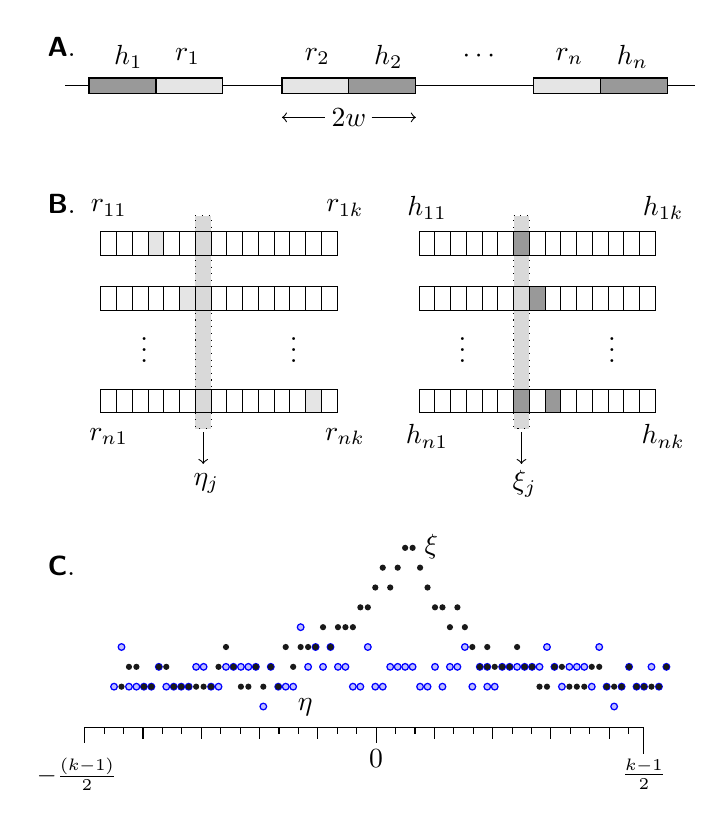
\begin{tikzpicture}
 %
 %------------------------------------------------------------------------
 %% hotspot + reference regions
 %------------------------------------------------------------------------
 % \begin{pgfonlayer}{background}
 %   \filldraw [line width=0.1mm, join=round, black, dashed]
 %       (-0.4,0.8)  rectangle (8.1,-0.8);
 % \end{pgfonlayer} 
 \node at (-0.05,0.5) {\textsf{\textbf{A}}.};
 \draw (0,0) -- (8,0);
 \draw[fill=black!40] (0.3, -0.1) -- (1.15,-0.1) -- (1.15,0.1) -- (0.3,0.1) -- cycle;
 \draw[fill=black!10] (1.15,-0.1) -- (2,-0.1) -- (2,0.1) -- (1.15,0.1) -- cycle;
 \draw[fill=black!10] (5.95,-0.1) -- (6.8,-0.1) -- (6.8,0.1) -- (5.95,0.1) -- cycle;
 \draw[fill=black!40] (6.8, -0.1) -- (7.65,-0.1) -- (7.65,0.1) -- (6.8,0.1) -- cycle;
 \draw[fill=black!10] (2.75,-0.1) -- (3.6,-0.1) -- (3.6,0.1) -- (2.75,0.1) -- cycle;
 \draw[fill=black!40] (3.6, -0.1) -- (4.45,-0.1) -- (4.45,0.1) -- (3.6,0.1) -- cycle;
 % labels
 \node at (0.8,0.37) {$h_1$};
 \node at (1.55,0.37)  {$r_1$};
 \node at (4.1,0.37)  {$h_2$};
 \node at (3.2,0.37) {$r_2$};
 \node at (5.25,0.37)  {$\cdots$};
 \node at (6.4,0.37)  {$r_n$};
 \node at (7.2,0.37)  {$h_n$};
 %
 \draw[<-] (2.75,-0.4) -- (3.3,-0.4);
 \draw[->] (3.89,-0.4) -- (4.45,-0.4);
 \node at (3.6,-0.4) {$2w$};
 %------------------------------------------------------------------------
 %% Matrizes of counts
 %------------------------------------------------------------------------
 %\begin{pgfonlayer}{background}
 %  \draw [line width=0.1mm, join=round, black, dashed]
 %      (-0.4,-1.2)  rectangle (8.1,-5.4);
 %\end{pgfonlayer} 
 %
 %% The r_{ij} matrix
 %
 \node at (-0.05,-1.5) {\textsf{\textbf{B}}.};
 \begin{scope}[yshift=-10pt]
  % vertical rectangle
  \draw[dotted, fill=black!15] (1.65,-1.3) -- (1.85,-1.3) -- (1.85, -4) -- (1.65, -4) -- cycle;
  % rows
  \draw (0.45, -1.5) -- (3.45, -1.5) -- (3.45, -1.8) -- (0.45, -1.8) -- cycle;
  \foreach \x in {0.45, 0.65,..., 3.35} {\draw (\x, -1.5) -- (\x, -1.8);}
  \draw[fill=black!10] (1.05, -1.5) -- (1.25, -1.5) -- (1.25, -1.8) -- (1.05, -1.8) -- cycle;
  %\draw[fill=black!10] (2.05, -1.5) -- (2.25, -1.5) -- (2.25, -1.8) -- (2.05, -1.8) -- cycle;
  \draw (0.45, -2.2) -- (3.45, -2.2) -- (3.45, -2.5) -- (0.45, -2.5) -- cycle;
  \foreach \x in {0.45, 0.65,..., 3.35} {\draw (\x, -2.2) -- (\x, -2.5);}
  \draw[fill=black!10] (1.45, -2.2) -- (1.65, -2.2) -- (1.65, -2.5) -- (1.45, -2.5) -- cycle;
  \node at (2.9, -2.9) {$\vdots$};
  \node at (1, -2.9) {$\vdots$};
  \draw (0.45, -3.5) -- (3.45, -3.5) -- (3.45, -3.8) -- (0.45, -3.8) -- cycle;
  \foreach \x in {0.45, 0.65,..., 3.35} {\draw (\x, -3.5) -- (\x, -3.8);}
  \draw[fill=black!10] (3.05, -3.5) -- (3.25, -3.5) -- (3.25, -3.8) -- (3.05, -3.8) -- cycle;
  \draw[->] (1.75, -4.05) -- (1.75, -4.45);
  % labels
  \node at (1.79, -4.7) {$\eta_j$};
  \node at (0.55, -1.2) {$r_{11}$};
  \node at (3.55, -1.2) {$r_{1k}$};
  \node at (0.55, -4.1) {$r_{n1}$};
  \node at (3.55, -4.1) {$r_{nk}$};
  % border
  %\draw[dashed] (0.3,-1.3) -- (3.6,-1.3) -- (3.6, -4) -- (0.3, -4) -- cycle;
 \end{scope}
 %
 %% The h_{ij} matrix
 %
 \begin{scope}[yshift=-10pt, xshift=115pt]
  % vertical rectangle
  \draw[dotted, fill=black!15] (1.65,-1.3) -- (1.85,-1.3) -- (1.85, -4) -- (1.65, -4) -- cycle;
  % rows
  \draw (0.45, -1.5) -- (3.45, -1.5) -- (3.45, -1.8) -- (0.45, -1.8) -- cycle;
  \foreach \x in {0.45, 0.65,..., 3.35} {\draw (\x, -1.5) -- (\x, -1.8);}
  \draw[fill=black!40] (1.65, -1.5) -- (1.85, -1.5) -- (1.85, -1.8) -- (1.65, -1.8) -- cycle;
  \draw (0.45, -2.2) -- (3.45, -2.2) -- (3.45, -2.5) -- (0.45, -2.5) -- cycle;
  \foreach \x in {0.45, 0.65,..., 3.35} {\draw (\x, -2.2) -- (\x, -2.5);}
  \draw[fill=black!40] (1.85, -2.2) -- (2.05, -2.2) -- (2.05, -2.5) -- (1.85, -2.5) -- cycle;
  \node at (2.9, -2.9) {$\vdots$};
  \node at (1, -2.9) {$\vdots$};
  \draw (0.45, -3.5) -- (3.45, -3.5) -- (3.45, -3.8) -- (0.45, -3.8) -- cycle;
  \foreach \x in {0.45, 0.65,..., 3.35} {\draw (\x, -3.5) -- (\x, -3.8);}
  \draw[fill=black!40] (1.65, -3.5) -- (1.85, -3.5) -- (1.85, -3.8) -- (1.65, -3.8) -- cycle;
  \draw[fill=black!40] (2.05, -3.5) -- (2.25, -3.5) -- (2.25, -3.8) -- (2.05, -3.8) -- cycle;
  \draw[->] (1.75, -4.05) -- (1.75, -4.45);
  % labels
  \node at (1.79, -4.7) {$\xi_j$};
  \node at (0.55, -1.2) {$h_{11}$};
  \node at (3.55, -1.2) {$h_{1k}$};
  \node at (0.55, -4.1) {$h_{n1}$};
  \node at (3.55, -4.1) {$h_{nk}$};
 \end{scope}
 %------------------------------------------------------------------------
 %% Profiles
 %------------------------------------------------------------------------
 %
 %% The ``sum'' of all histograms
 %
 \node at (-0.05,-6.1) {\textsf{\textbf{C}}.};
 \begin{scope}[xshift=-30pt, yshift=30pt]
  \begin{axis}[
    width=10cm, height=4cm,
    at={(0.08\linewidth,-260pt)},
    hide x axis,
    hide y axis,
    mark size = 2pt % set to 0pt to have no mark
    ]
  \addplot+[only marks, mark=*, draw=blue, every mark/.append style={scale=0.6, fill=blue!25, line width=0.45pt}]%
   coordinates {
    (-10,0) (-9,2) (-8,0) (-7,0) (-6,0)  
    (-5,0) (-4,1) (-3,0) (-2,0) (-1,0)
    (0,0)  (1,1) (2,1) (3,0) (4,0) (5,1) 
    (6,1) (7,1) (8,1) (9,1) (10,-1) 
    (11,1) (12,0) (13,0) (14,0) (15,3) 
    (16,1) (17,2) (18,1) (19,2) (20,1) 
    (21,1) (22,0) (23,0) (24,2) (25,0) 
    (26,0) (27,1) (28,1) (29,1) (30,1)
    (31,0) (32,0) (33,1) (34,0) (35,1)
    (36,1) (37,2) (38,0) (39,1) (40,1)
    (40,0) (41,0) (42,1) (43,1) (44,1) 
    (45,1) (46,1) (47,1) (48,2) (49,1) 
    (50,0) (51,1) (52,1) (53,1) (54,0)
    (55,2) (56,0) (57,-1) (58,0) (59,1)
    (60,0) (61,0) (62,1) (63,0) (64,1)

 };
  \addplot+[only marks, mark=*, draw=black!90, every mark/.append style={scale=0.425, fill=black!90, line width=0.5pt}]%
   coordinates {
     (-9,0) (-8,1) (-7,1) (-6,0) (-5,0) 
    (-4,1) (-3,1) (-2,0) (-1,0) (0,0) 
    (1,0) (2,0) (3,0) (4,1) (5,2) 
    (6,1) (7,0) (8,0) (9,1) (10,0) 
    (11,1) (12,0) (13,2) (14,1) (15,2) 
    (16,2) (17,2) (18,3) (19,2) (20,3) 
    (21,3) (22,3) (23,4) (24,4) (25,5) 
    (26,6) (27,5) (28,6) (29,7) (30,7)
    (31,6) (32,5) (33,4) (34,4) (35,3)
    (36,4) (37,3) (38,2) (39,1) (40,2)
    (40,1) (41,1) (42,1) (43,1) (44,2) 
    (45,1) (46,1) (47,0) (48,0) (49,1) 
    (50,1) (51,0) (52,0) (53,0) (54,1) 
    (55,1) (56,0) (57,0) (58,0) (59,1)
    (60,0) (61,0) (62,0) (63,0) (64,1)
  };
 \end{axis}
 \node at (5.7, -6.9) {$\xi$};
 \node at (4.1,-8.95) {$\eta$};

 \draw (1.3,-9.2) -- (8.4,-9.2);
  
  \draw (1.3, -9.2) -- (1.3, -9.4);
  \draw (5, -9.2) -- (5, -9.4);
  \draw (8.4, -9.2) -- (8.4, -9.54);
  
  \node at (5, -9.6) {0};
  \node at (1.2, -9.8) {\small $-\frac{(k-1)}{2}$};
  \node at (8.4, -9.8) {\small $\frac{k-1}{2}$};
  \foreach \x in {1.3, 2.04,..., 8.4} {\draw (\x, -9.2) -- (\x, -9.35);}
  \foreach \x in {1.3, 1.54666,..., 8.4} {\draw (\x, -9.2) -- (\x, -9.28);}
 \end{scope}
\end{tikzpicture}